Abbildungen der Messreihen mit verschiedenen Spannungen bei Abständen von ein bis fünf Metern.
\begin{minipage}{0.5\textwidth}
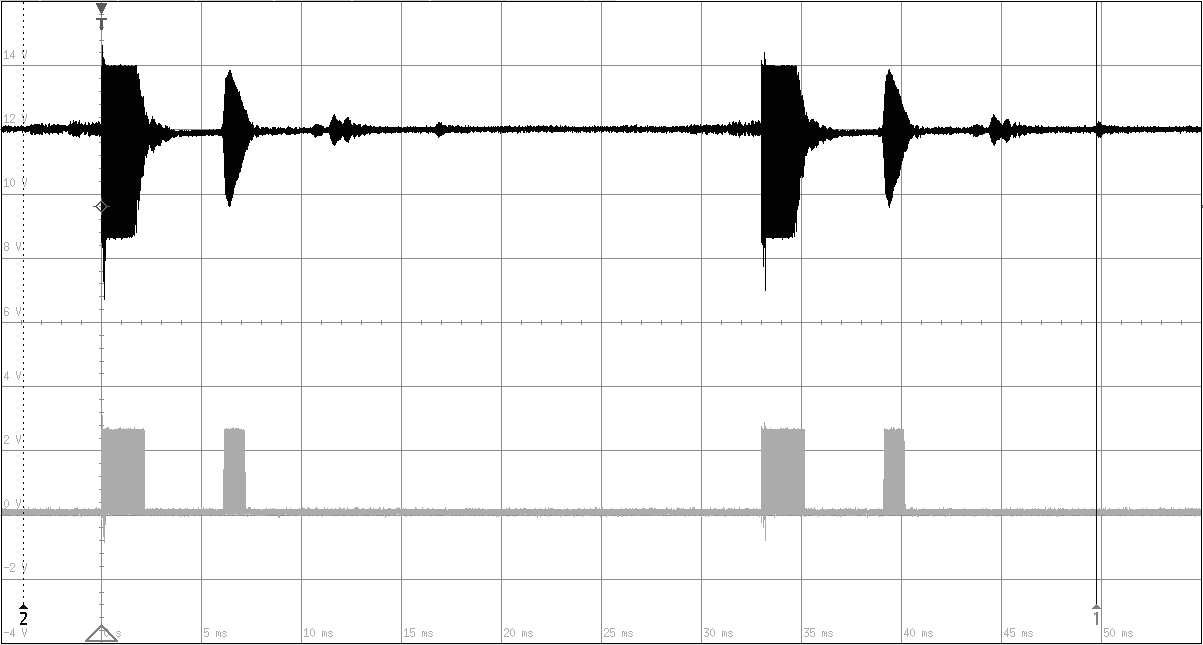
\includegraphics[width=1\textwidth%, draft
]{Abbildungen/MessungenP2/5V/1m.PNG}
\captionof{figure}{Signalverlauf bei 5V auf 1m Abstand}
\end{minipage}
\begin{minipage}{0.5\textwidth}
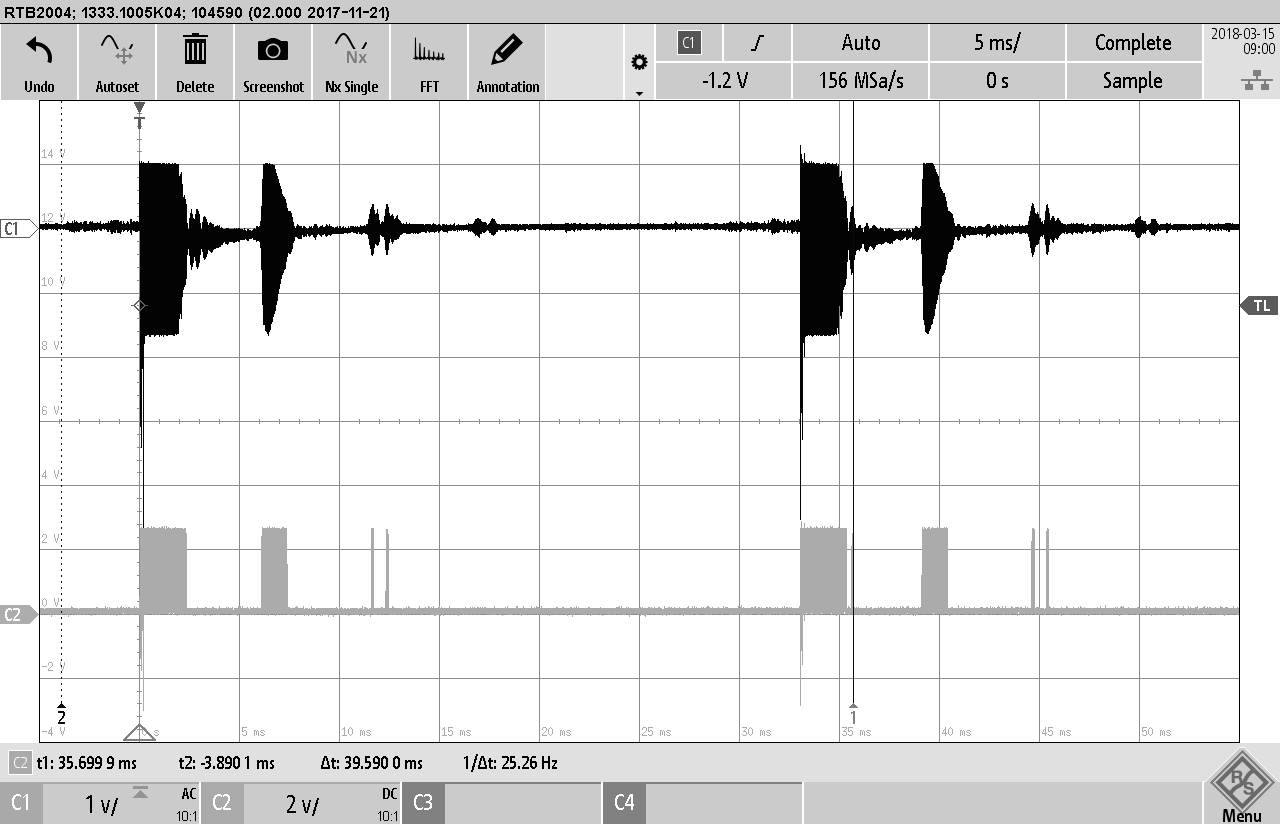
\includegraphics[width=1\textwidth%, draft
]{Abbildungen/MessungenP2/10V/1m.PNG}
\captionof{figure}{Signalverlauf bei 10V auf 1m Abstand}
\end{minipage}
\begin{minipage}{0.5\textwidth}
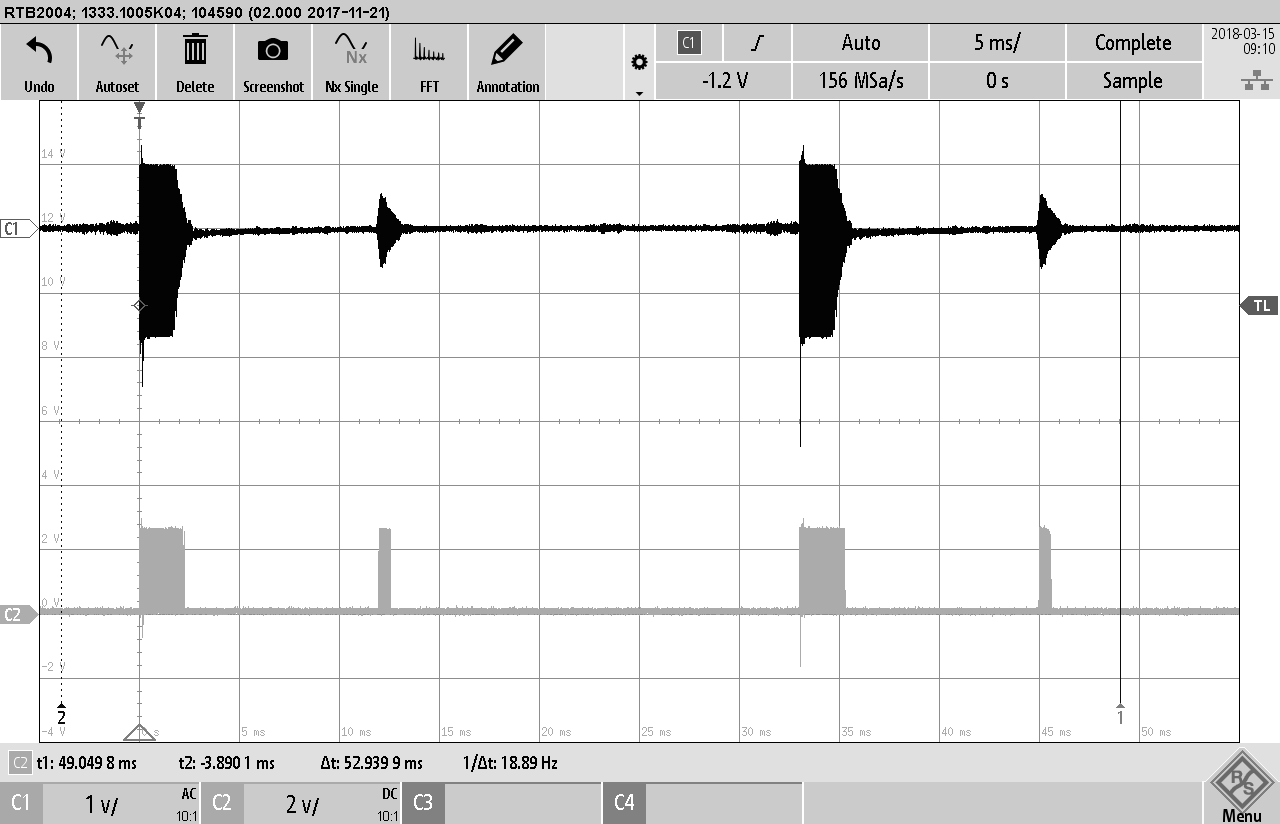
\includegraphics[width=1\textwidth%, draft
]{Abbildungen/MessungenP2/5V/2m.PNG}
\captionof{figure}{Signalverlauf bei 5V auf 2m Abstand}
\end{minipage}
\begin{minipage}{0.5\textwidth}
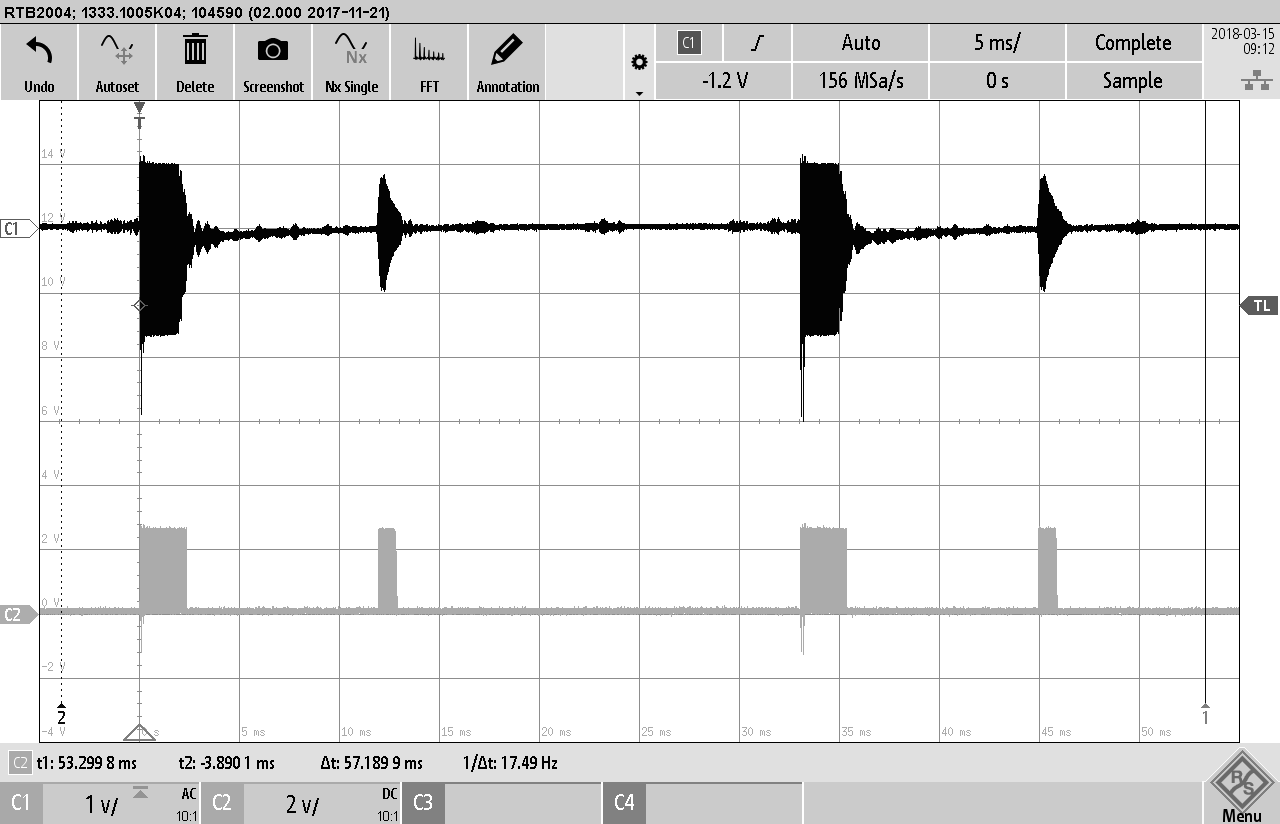
\includegraphics[width=1\textwidth%, draft
]{Abbildungen/MessungenP2/10V/2m.PNG}
\captionof{figure}{Signalverlauf bei 10V auf 2m Abstand}
\end{minipage}
\begin{minipage}{0.5\textwidth}
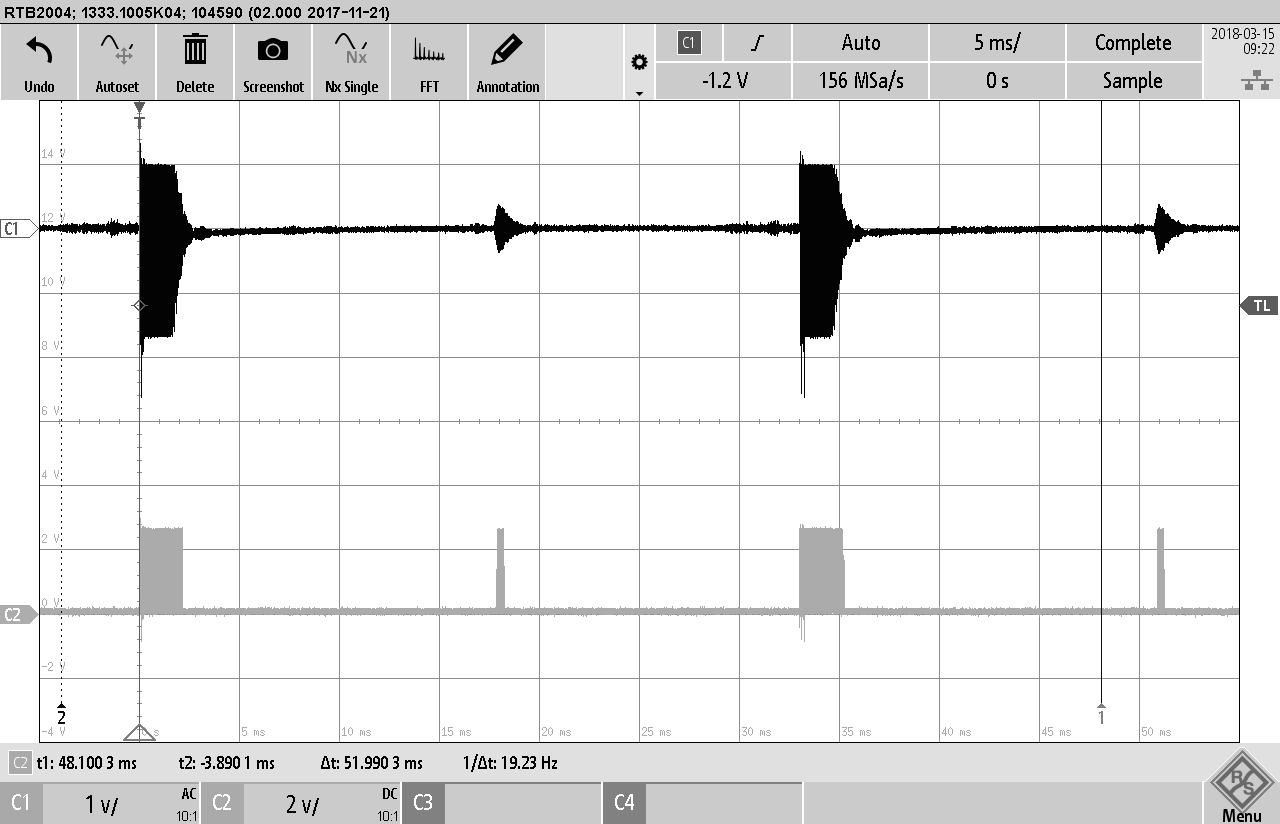
\includegraphics[width=1\textwidth%, draft
]{Abbildungen/MessungenP2/5V/3m.PNG}
\captionof{figure}{Signalverlauf bei 5V auf 3m Abstand}
\end{minipage}
\begin{minipage}{0.5\textwidth}
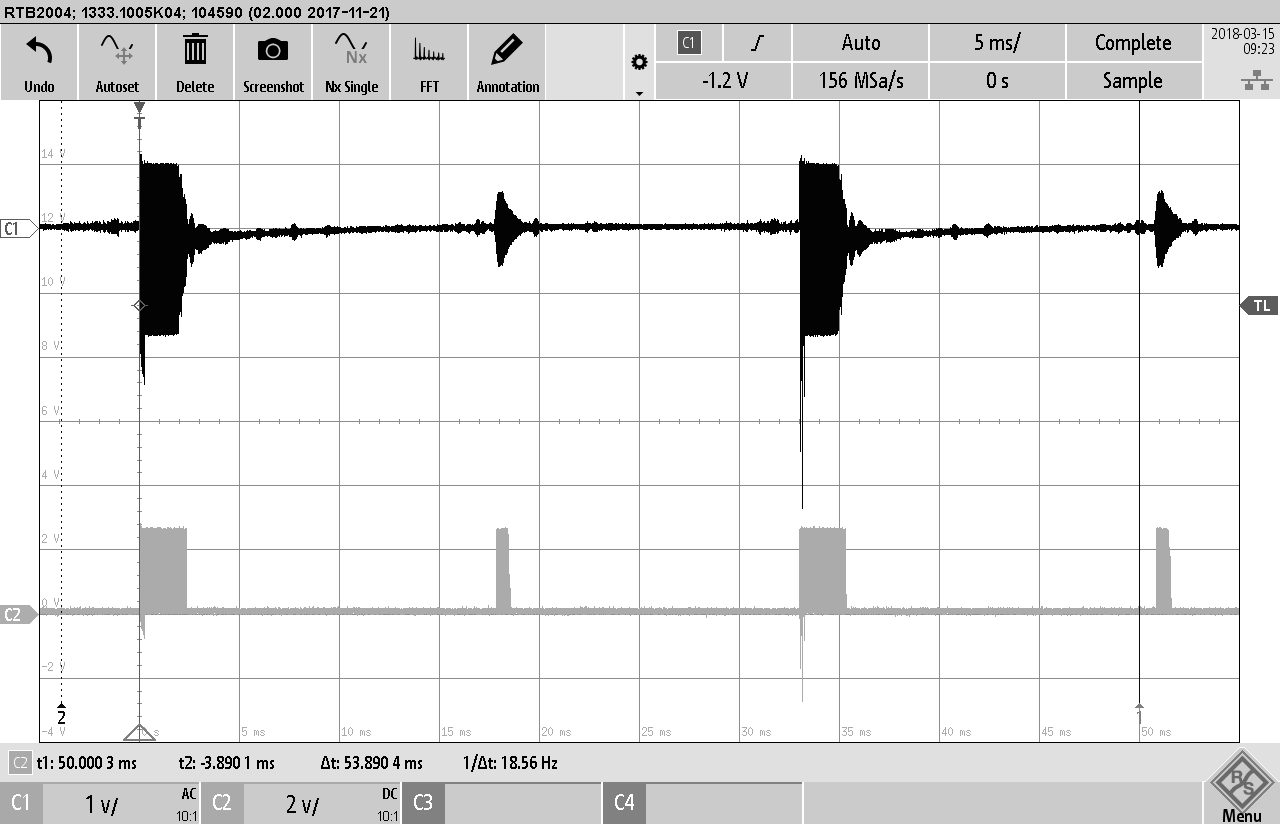
\includegraphics[width=1\textwidth%, draft
]{Abbildungen/MessungenP2/10V/3m.PNG}
\captionof{figure}{Signalverlauf bei 10V auf 3m Abstand}
\end{minipage}
\begin{minipage}{0.5\textwidth}
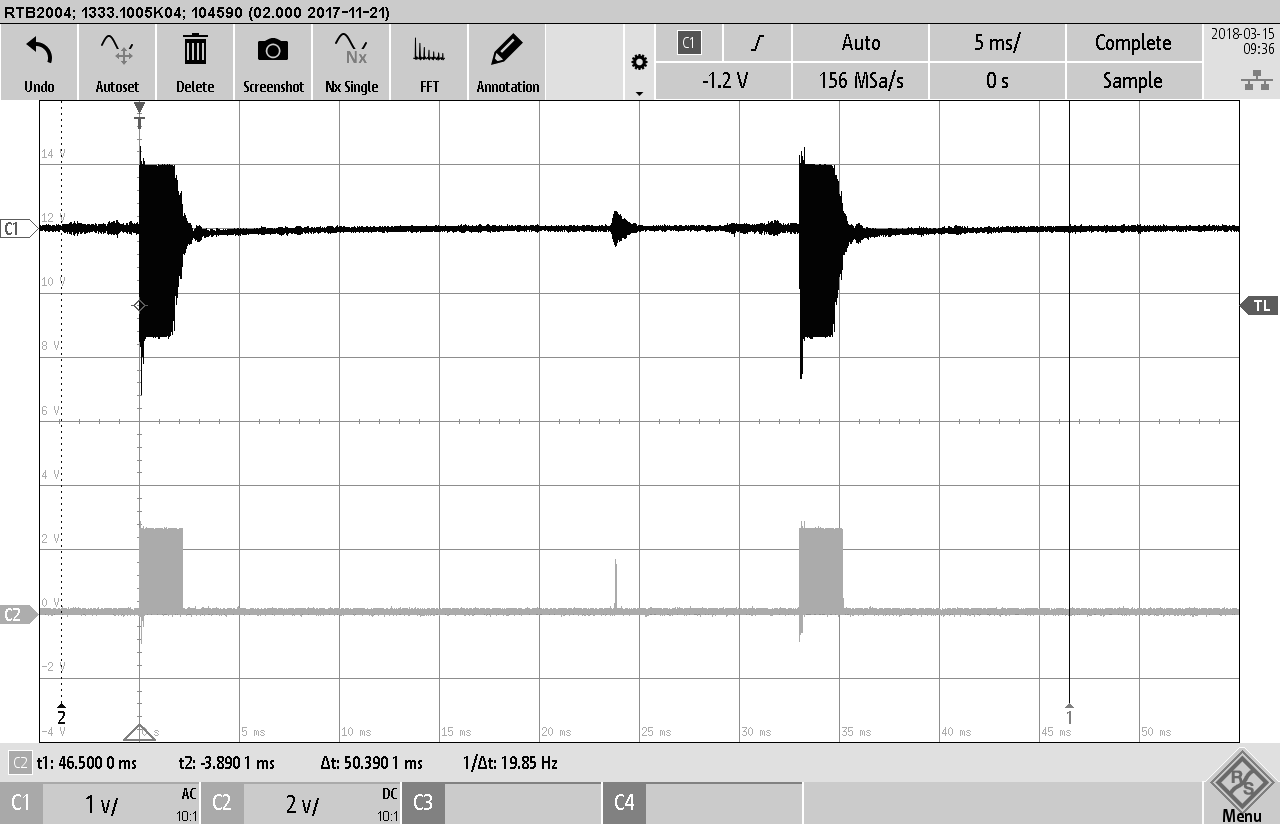
\includegraphics[width=1\textwidth%, draft
]{Abbildungen/MessungenP2/5V/4m.PNG}
\captionof{figure}{Signalverlauf bei 5V auf 4m Abstand}
\end{minipage}
\begin{minipage}{0.5\textwidth}
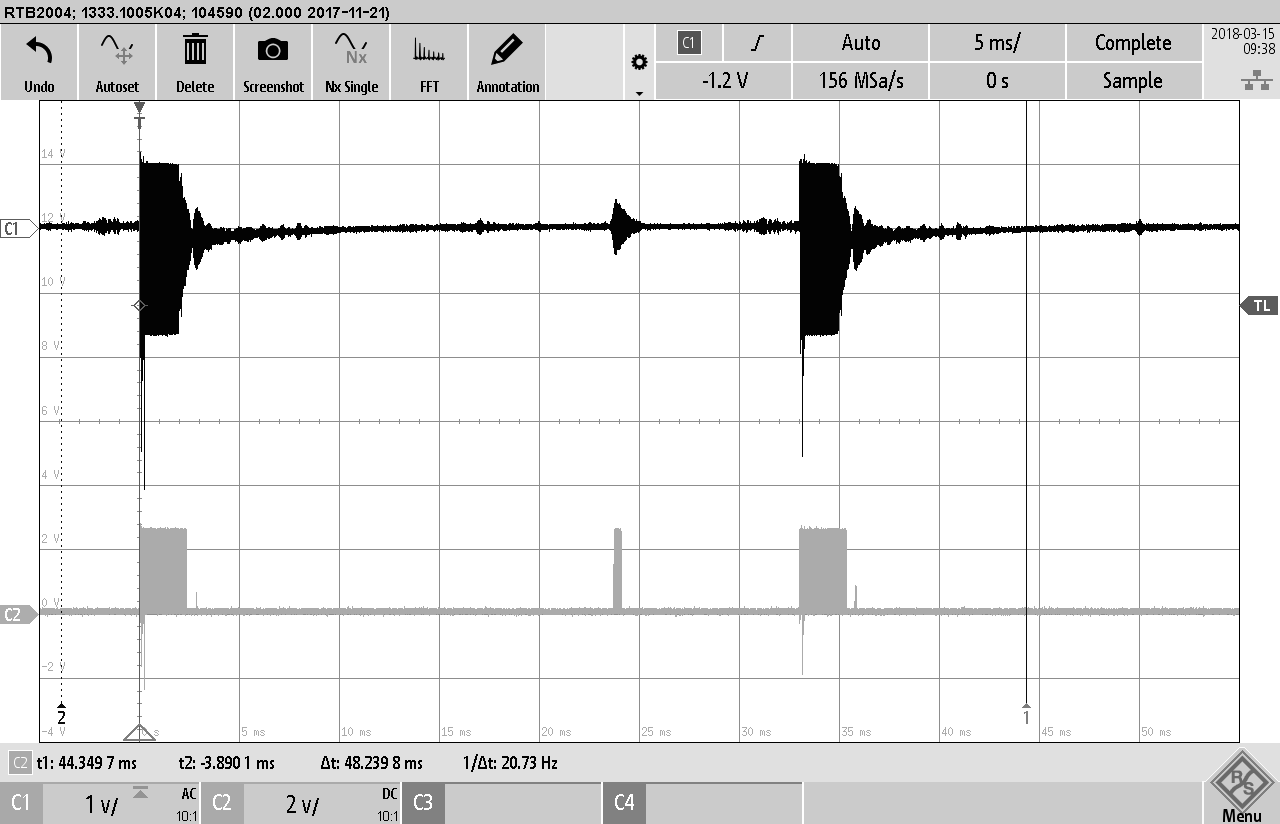
\includegraphics[width=1\textwidth%, draft
]{Abbildungen/MessungenP2/10V/4m.PNG}
\captionof{figure}{Signalverlauf bei 10V auf 4m Abstand}
\end{minipage}
\begin{minipage}{0.5\textwidth}
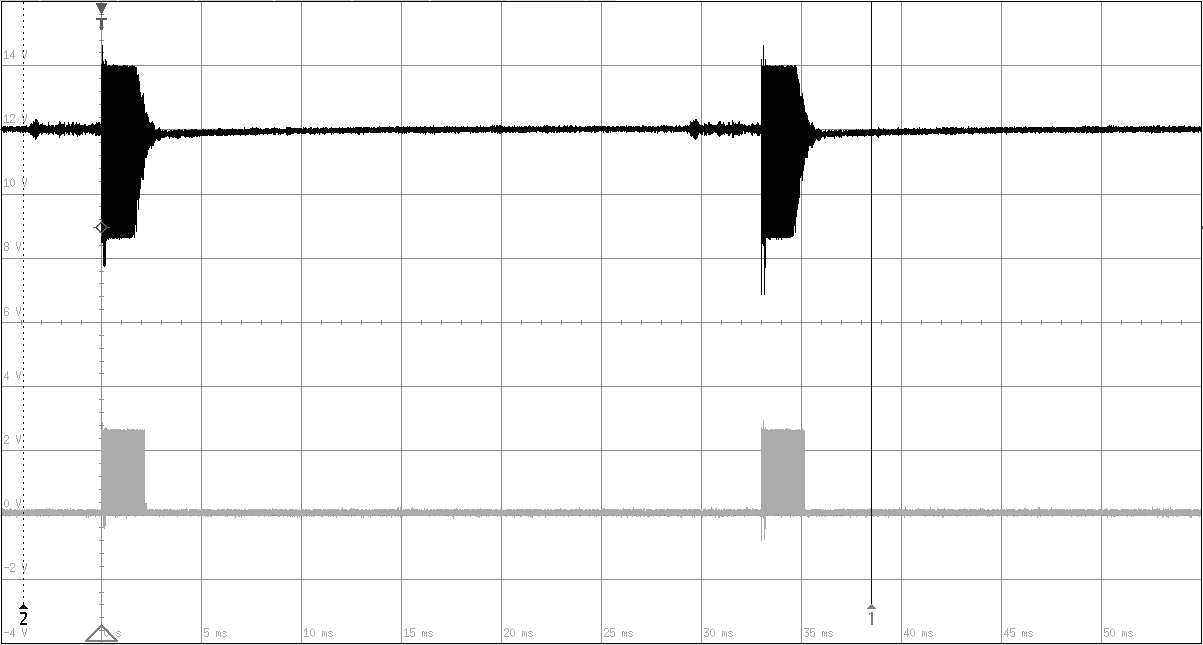
\includegraphics[width=1\textwidth%, draft
]{Abbildungen/MessungenP2/5V/5m.PNG}
\captionof{figure}{Signalverlauf bei 5V auf 5m Abstand}
\end{minipage}
\begin{minipage}{0.5\textwidth}
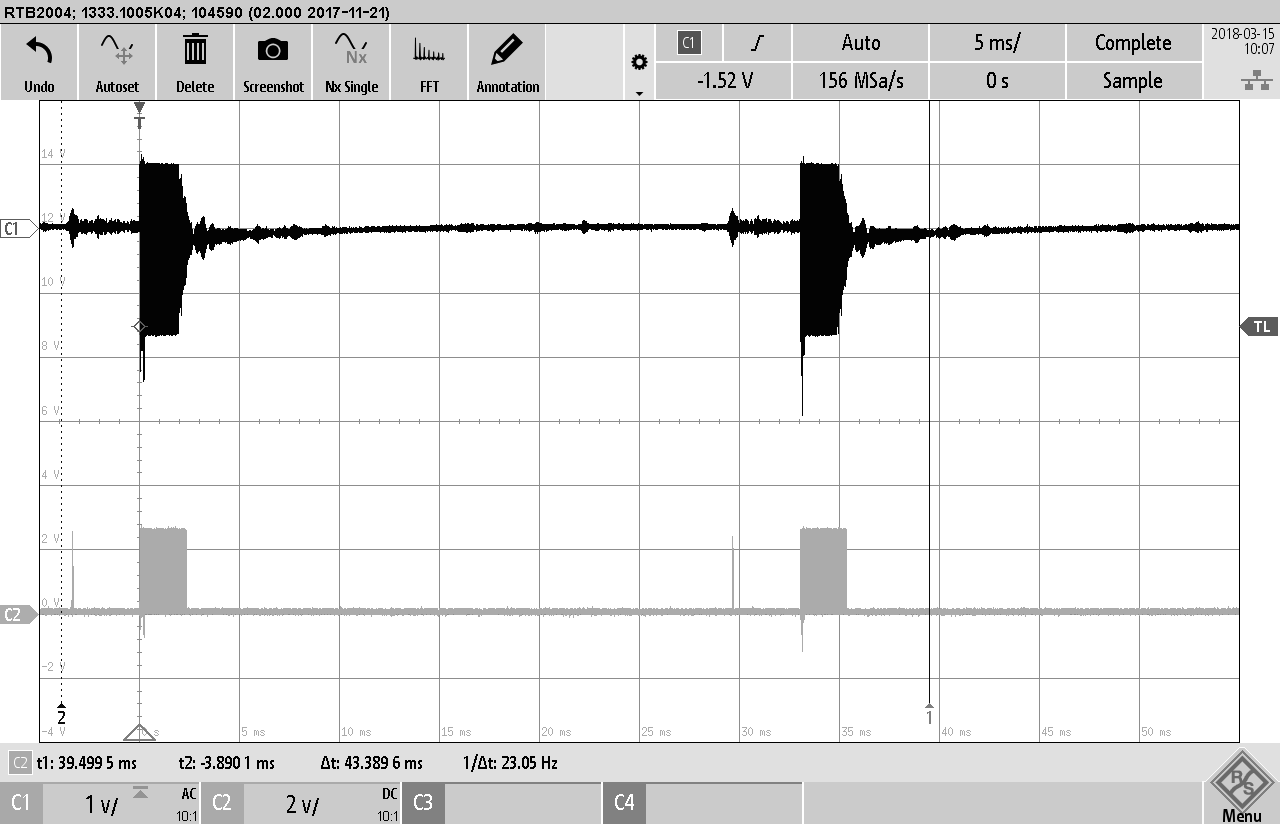
\includegraphics[width=1\textwidth%, draft
]{Abbildungen/MessungenP2/10V/5m.PNG}
\captionof{figure}{Signalverlauf bei 10V auf 5m Abstand}
\end{minipage}

\begin{minipage}{1\textwidth}
\begin{tabularx}{\textwidth}{|p{0.1\textwidth}|p{0.2\textwidth}|p{0.2\textwidth}|p{0.2\textwidth}|X|}
\hline
Entfernung [m]& Zeit bis Anfang Echo [ms] & Zeit bis Ende Echo [ms] & Errechnete Entfernung Anfang [m] & Errechnete Entfernung Ende [m]\\
\hline
1 & 6,11 & 7,23 & 1,0485 & 1,2407\\
\hline
1,5 & 9,02 & 9,89 & 1,5478 & 1,6971\\
\hline
2 & 11,97 & 12,76 & 2,0541 & 2,1896\\
\hline
2,5 & 14,88 & 15,5 & 2,5534 & 2,659\\
\hline
3 & 17,84 & 18,2 & 3,06134 & 3,1231\\
\hline
3,5 & 20,8 & 21,11 & 3,569 & 3,6225\\
\hline
4 & 23,71 & 23,81 & 4,0686 & 4,0858\\
\hline
4,5 & 26,61 & 26,73 & 4,5663 & 4,5869\\
\hline
5 & 29,59 & 29,68 & 5,0776 & 5,0961\\
\hline
\end{tabularx}
\captionof{table}{Entfernungsmessung bei 5V Sendespannung}
\label{tab:Entfernungsmessung5V}
\begin{tabularx}{\textwidth}{|p{0.1\textwidth}|p{0.2\textwidth}|p{0.2\textwidth}|p{0.2\textwidth}|X|}
\hline
Entfernung [m]& Zeit bis Anfang Echo [ms] & Zeit bis Ende Echo [ms] & Errechnete Entfernung Anfang [m] & Errechnete Entfernung Ende [m]\\
\hline
1 & 6,07 & 7,37 & 1,0416 & 1,2647\\
\hline
1,5 & 8,99 & 10,02 & 1,5427 & 1,7194\\
\hline
2 & 11,94 & 12,9 & 2,0489 & 2,2136\\
\hline
2,5 & 14,83 & 15,7 & 2,5448 & 2,6941\\
\hline
3 & 17,8 & 18,48 & 3,0545 & 3,1712\\
\hline
3,5 & 20,7 & 21,36 & 3,5521 & 3,6654\\
\hline
4 & 23,62 & 24 & 4,0532 & 4,1184\\
\hline
4,5 & 26,55 & 26,9 & 4,5560 & 4,6160\\
\hline
5 & 29,5 & 29,9 & 5,0622 & 5,1308\\
\hline
\end{tabularx}
\captionof{table}{Entfernungsmessung bei 10V Sendespannung}
\label{tab:Entfernungsmessung10V}
\end{minipage}\\